\documentclass[aspectratio=169, 10pt]{beamer}

\usetheme{Madrid}
\usecolortheme{whale}

\usepackage{amsmath,amssymb,amsfonts}
\usepackage{booktabs}
\usepackage{graphicx}
\usepackage{tikz}
\usetikzlibrary{shapes.geometric, arrows.meta, positioning, calc, fit}
\usepackage{xcolor}

% Custom Colors matching ISMLL / academic styling
\definecolor{primaryblue}{RGB}{24, 76, 120}
\definecolor{accentorange}{RGB}{214, 90, 49}
\definecolor{darkgray}{RGB}{45, 52, 54}
\definecolor{lightgray}{RGB}{245, 246, 250}
\definecolor{successgreen}{RGB}{46, 117, 89}

\setbeamercolor{palette primary}{bg=primaryblue,fg=white}
\setbeamercolor{palette secondary}{bg=primaryblue!85,fg=white}
\setbeamercolor{palette tertiary}{bg=primaryblue!70,fg=white}
\setbeamercolor{structure}{fg=primaryblue}
\setbeamercolor{frametitle}{bg=primaryblue,fg=white}
\setbeamercolor{title}{bg=primaryblue,fg=white}

\setbeamertemplate{navigation symbols}{}
\setbeamertemplate{footline}[frame number]

\title[\textbf{Lightweight MTS Forecasting: CycleNet-Pro}]{\textbf{Spectral Integrity, Modular Backbones, and Boundary Conditions in Lightweight Time Series Forecasting}}
\subtitle{Mid-Term Defense: Progress, Automated Recurrent Periodicity, and Empirical Diagnostics}
\author[Chaturvedi et al.]{\textbf{Aaditya Chaturvedi} \and \textbf{Abdelhadi Hadj Sahraoui} \and \textbf{Philip Gentner} \and \textbf{Mohamad Taleb} \\ \vspace{0.15cm}\small Supervisor: Jung Min Choi}
\institute[Univ.~Hildesheim]{Information Systems and Machine Learning Lab (ISMLL) \\ Institute for Computer Science, University of Hildesheim, Germany}
\date{September 2026}

\begin{document}

% =========================================================================
% SLIDE 1: Title Slide
% =========================================================================
\begin{frame}
  \titlepage
\end{frame}

% =========================================================================
% SLIDE 2: Research Motivation & Problem Statement
% =========================================================================
\begin{frame}{1. The Lightweight Forecasting Revolution: Promise \& Flaws}
\begin{columns}[T]
\column{0.55\textwidth}
\textbf{The Transformer vs. Linear Paradigm Shift:}
\begin{itemize}
    \item Multi-head attention architectures (Autoformer, PatchTST) established SOTA accuracy but carry heavy compute/memory footprints.
    \item \textbf{DLinear (Zeng et al., AAAI 2023)} proved that simple moving-average decomposition matches or outperforms Transformers with $100\times$ fewer parameters.
\end{itemize}
\vspace{0.3cm}
\textbf{The Unaddressed Research Question:}
\begin{block}{Supervisor Mandate (Jung Min Choi)}
\textit{"When does frequency-domain and periodic modeling actually help versus fail in lightweight MTS forecasting?"}
\end{block}

\column{0.45\textwidth}
\begin{alertblock}{The Failure Mode of Moving Averages}
\begin{itemize}
    \item Naive moving-average trends diverge catastrophically on non-stationary shifts over long horizons ($H=720$ on ETTh2).
    \item Averages act as low-pass filters, dampening sharp periodic peaks and distorting harmonic phase.
\end{itemize}
\end{alertblock}
\end{columns}
\end{frame}

% =========================================================================
% SLIDE 3: The Spectral Masking Problem
% =========================================================================
\begin{frame}{2. The Core Problem: Why Scalar MSE Lies}
\begin{columns}[T]
\column{0.50\textwidth}
\textbf{The Deception of Scalar Metrics:}
\begin{itemize}
    \item Standard benchmarks evaluate models strictly via aggregate time-domain metrics: Mean Squared Error (MSE) and Mean Absolute Error (MAE).
    \item Under unconstrained $\ell_2$ loss optimization, linear layers take numerical shortcuts: predicting the conditional mean of rapid oscillations depresses aggregate MSE.
    \item \textbf{Consequence:} Models show "good" MSE while severely attenuating physical cyclic harmonics (over-smoothing).
\end{itemize}

\column{0.50\textwidth}
\begin{block}{Real-World Physical Telemetry Decomposition}
Telemetry is a superposition of distinct physical phenomena:
\begin{enumerate}
    \item \textbf{Low-Frequency ($\mathcal{B}_{\text{low}}$):} Secular trend, seasonal drift ($T \ge 10\text{ h}$).
    \item \textbf{Mid-Frequency ($\mathcal{B}_{\text{mid}}$):} Physical periodic cycles (diurnal solar, intra-day demand, $2.5\text{ h} \le T < 10\text{ h}$).
    \item \textbf{High-Frequency ($\mathcal{B}_{\text{high}}$):} Stochastic perturbations, sensor noise ($2.0\text{ h} \le T < 2.5\text{ h}$).
\end{enumerate}
\end{block}
\end{columns}
\end{frame}

% =========================================================================
% SLIDE 4: Diagnostic Apparatus: Exact Parseval Decomposition
% =========================================================================
\begin{frame}{3. Diagnostic Framework: Energy-Conserving Parseval Decomposition}
To diagnose structural fidelity without filtering artifacts, we formulate an exact subband decomposition via Parseval's Theorem on one-sided rFFT:
\begin{equation*}
    \sum_{t=0}^{H-1} |e(t)|^2 = \frac{1}{H} \sum_{k=0}^{H-1} |E(k)|^2 \implies \text{MSE}_{\text{total}} = \frac{1}{H^2} \sum_{k=0}^{\lfloor H/2 \rfloor} w_k |E(k)|^2
\end{equation*}

\vspace{0.2cm}
\begin{columns}[T]
\column{0.6\textwidth}
\textbf{Exact Physical Frequency Partitioning ($f = k/H$):}
\begin{itemize}
    \item $\mathcal{B}_{\text{low}} = [0, 0.1)$: Macro-trend \& baseline drift ($T \ge 10\text{ h}$).
    \item $\mathcal{B}_{\text{mid}} = [0.1, 0.4)$: Harmonic intra-day cyclic dynamics.
    \item $\mathcal{B}_{\text{high}} = [0.4, 0.5]$: Stochastic micro-fluctuations \& noise.
\end{itemize}
\begin{block}{Mathematical Exactness}
$\text{MSE}_{\text{total}} \equiv \text{MSE}_{\text{low}} + \text{MSE}_{\text{mid}} + \text{MSE}_{\text{high}}$ (Zero energy leakage).
\end{block}

\column{0.4\textwidth}
\begin{exampleblock}{Subband Metric Properties}
\begin{itemize}
    \item \textbf{Exact Identity}: No heuristics or window leakage.
    \item \textbf{Failure Localization}: Isolates whether error stems from drifting trend, damped harmonics, or noise amplification.
\end{itemize}
\end{exampleblock}
\end{columns}
\end{frame}

% =========================================================================
% SLIDE 5: Normalized Diagnostics: FVU and LSD
% =========================================================================
\begin{frame}{4. Normalized Frequency Metrics: Scale-Free Diagnostics}
Because raw MSE is scale-dependent, we establish two physical diagnostic metrics:
\vspace{0.2cm}
\begin{columns}[T]
\column{0.50\textwidth}
\textbf{1. Fraction of Variance Unexplained ($FVU_{\text{band}}$):}
\begin{equation*}
    FVU_{\text{band}} = \frac{\sum_{k \in \mathcal{B}} w_k |E(k)|^2}{\sum_{k \in \mathcal{B}} w_k |Y(k) - \bar{Y}(k)|^2}
\end{equation*}
\begin{itemize}
    \item $FVU < 1.0$: Model learns genuine physical dynamics in that band.
    \item $FVU \approx 1.0$: Model performs no better than predicting a flat mean line.
    \item $FVU > 1.0$: Model actively hallucinates power and amplifies noise.
\end{itemize}

\column{0.50\textwidth}
\textbf{2. Log-Spectral Distance (LSD in dB):}
\begin{equation*}
    \text{LSD} = \sqrt{\frac{1}{M} \sum_{k=0}^{M-1} \left( 10 \log_{10} \frac{|\hat{Y}(k)|^2 + \epsilon}{|Y(k)|^2 + \epsilon} \right)^2}
\end{equation*}
\begin{itemize}
    \item Quantifies perceptual power spectral density (PSD) distortion across the full Nyquist range.
    \item Directly penalizes harmonic damping and spectral collapse.
\end{itemize}
\end{columns}
\end{frame}

% =========================================================================
% SLIDE 6: Automated CycleNet-Pro Overview
% =========================================================================
\begin{frame}{5. Proposed Solution: Automated CycleNet (CycleNet-Pro)}
\begin{center}
\textbf{Core Concept: Explicit Periodic Memory + Modular Residual Backbones}
\end{center}
\vspace{-0.2cm}
\begin{columns}[T]
\column{0.52\textwidth}
\begin{enumerate}
    \item \textbf{RevIN Instance Normalization}: Guards against global non-stationary distribution shifts.
    \item \textbf{Automated Period Discovery}: Dynamically extracts multi-period cycles via FFT + ACF (no hardcoded periods).
    \item \textbf{Recurrent Cyclic State Queues}: Maintains explicit learnable periodic parameters $\mathbf{Q}^{(k)}$.
    \item \textbf{Modular Residual Backbones}: De-cycles inputs and routes residuals through specialized backbones.
    \item \textbf{Residual Channel Mixing}: Selectively mixes inter-channel dependencies only when correlated.
\end{enumerate}

\column{0.48\textwidth}
\begin{figure}
\centering
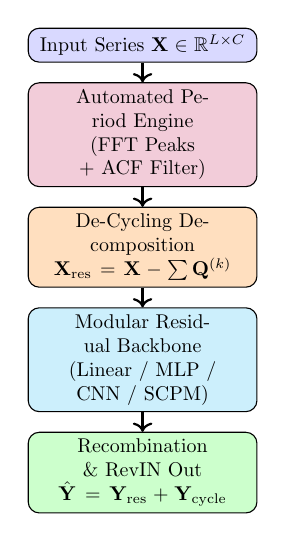
\begin{tikzpicture}[scale=0.72, every node/.style={transform shape}]
    \node[draw, rounded corners, fill=blue!15, text width=3.8cm, align=center] (inp) {Input Series $\mathbf{X} \in \mathbb{R}^{L \times C}$};
    \node[draw, rounded corners, fill=purple!20, below=0.35cm of inp, text width=3.8cm, align=center] (det) {Automated Period Engine\\(FFT Peaks + ACF Filter)};
    \node[draw, rounded corners, fill=orange!25, below=0.35cm of det, text width=3.8cm, align=center] (dec) {De-Cycling Decomposition\\$\mathbf{X}_{\text{res}} = \mathbf{X} - \sum \mathbf{Q}^{(k)}$};
    \node[draw, rounded corners, fill=cyan!20, below=0.35cm of dec, text width=3.8cm, align=center] (bb) {Modular Residual Backbone\\(Linear / MLP / CNN / SCPM)};
    \node[draw, rounded corners, fill=green!20, below=0.35cm of bb, text width=3.8cm, align=center] (rec) {Recombination \& RevIN Out\\$\hat{\mathbf{Y}} = \mathbf{Y}_{\text{res}} + \mathbf{Y}_{\text{cycle}}$};
    \draw[->, thick] (inp) -- (det);
    \draw[->, thick] (det) -- (dec);
    \draw[->, thick] (dec) -- (bb);
    \draw[->, thick] (bb) -- (rec);
\end{tikzpicture}
\end{figure}
\end{columns}
\end{frame}

% =========================================================================
% SLIDE 7: Automated Multi-Period Discovery Engine
% =========================================================================
\begin{frame}{6. Engine Stage 1: Automated Period Discovery (FFT + ACF)}
Prior models forced arbitrary hardcoded periodicities ($p=24$ or $p=96$). CycleNet-Pro discovers physical periods autonomously from training data:
\vspace{0.2cm}
\begin{columns}[T]
\column{0.33\textwidth}
\begin{block}{1. FFT Peak Ranking}
\begin{itemize}
    \item Compute power spectrum: $P(f) = |\text{rFFT}(\mathbf{x})|^2$.
    \item Extract candidate peaks via local extrema detection.
    \item Merge spectral leakage clusters within a 12\% relative distance.
\end{itemize}
\end{block}

\column{0.33\textwidth}
\begin{alertblock}{2. ACF Noise Filter}
\begin{itemize}
    \item Validate candidate periods using empirical Autocorrelation (ACF).
    \item 95\% white-noise confidence threshold:
    $$\text{Bound}_{\text{ACF}} = \frac{1.96}{\sqrt{N_{\text{train}}}}$$
    \item Eliminates spurious spectral peaks.
\end{itemize}
\end{alertblock}

\column{0.34\textwidth}
\begin{exampleblock}{3. Variance Decision}
\begin{itemize}
    \item Calculate marginal variance reduction of candidate cycles:
    $$\Delta \text{Var}(k) \ge 2.0\%$$
    \item Automatically accepts secondary/tertiary harmonics (e.g., intra-day + weekly cycles).
\end{itemize}
\end{exampleblock}
\end{columns}
\end{frame}

% =========================================================================
% SLIDE 8: Recurrent Memory Queues & De-Cycling
% =========================================================================
\begin{frame}{7. Engine Stage 2: Recurrent Periodic Queues \& De-Cycling}
\begin{columns}[T]
\column{0.55\textwidth}
\textbf{Explicit Recurrent State Formulation:}
\begin{itemize}
    \item For each discovered period $p_k \in \mathcal{P}$, maintain a learnable state matrix $\mathbf{Q}^{(k)} \in \mathbb{R}^{p_k \times C}$.
    \item Given global time index $\tau$, retrieve historical periodic pattern via circular phase indexing:
    \begin{equation*}
        \mathbf{C}^{(k)}_t = \mathbf{Q}^{(k)}_{(\tau + t) \pmod{p_k}}, \quad t \in [0, L-1]
    \end{equation*}
    \item \textbf{Residual De-Cycling:} Subtract periodic components from RevIN-normalized input:
    \begin{equation*}
        \mathbf{X}_{\text{res}} = \mathbf{X}_{\text{norm}} - \sum_{k=1}^K \mathbf{C}^{(k)}
    \end{equation*}
\end{itemize}

\column{0.45\textwidth}
\begin{block}{Why De-Cycling Works}
\begin{itemize}
    \item The residual $\mathbf{X}_{\text{res}}$ contains only non-periodic dynamics (secular trends, transient shocks, weather regime changes).
    \item The residual backbone does not waste capacity learning repetitive diurnal cycles.
    \item Periodic extrapolation to horizon $H$ is mathematically exact:
    $$\mathbf{Y}_{\text{cycle}, t} = \sum_{k=1}^K \mathbf{Q}^{(k)}_{(\tau + L + t) \pmod{p_k}}$$
\end{itemize}
\end{block}
\end{columns}
\end{frame}

% =========================================================================
% SLIDE 9: Modular Residual Backbones & SCPM Revision
% =========================================================================
\begin{frame}{8. Modular Residual Backbones: Specialization \& SCPM Revision}
CycleNet-Pro provides four modular, interchangeable residual backbones:
\vspace{0.15cm}
\begin{columns}[T]
\column{0.50\textwidth}
\begin{block}{1. Linear \& MLP Backbones}
\begin{itemize}
    \item \textbf{Linear}: Channel-independent $\mathbf{W} \in \mathbb{R}^{H \times L}$. Parameter-efficient baseline.
    \item \textbf{MLP}: 2-layer projection with hidden dimension 512 + GELU for non-linear temporal dynamics.
\end{itemize}
\end{block}
\begin{block}{2. 1D-CNN Backbone (Edge-Scale)}
\begin{itemize}
    \item Shared 1D-Conv across time and channels with linear length interpolation ($L \to H$).
    \item Slashes parameters by \textbf{97.7\%} (5.5k vs. 241k on ETT).
\end{itemize}
\end{block}

\column{0.50\textwidth}
\begin{exampleblock}{3. Revised SOR: SCPM Backbone}
\textbf{Spectral-Conditioned Patch Mixer (SCPM):}
\begin{itemize}
    \item \textbf{Intra-Patch Mixer}: Token MLP along time within each patch + feature MLP.
    \item \textbf{Inter-Patch Mixer}: Neighbor-aware gated MLP across local patch order + feature MLP.
    \item \textbf{FiLM Spectral Conditioning}: Reads orthonormal DCT-II log-energy subbands and dynamically modulates patch tokens:
    $$\mathbf{Z}_{\text{cond}} = \mathbf{Z} \odot (1 + \boldsymbol{\gamma}) + \boldsymbol{\beta}$$
    Zero-initialization ensures training starts strictly from identity.
\end{itemize}
\end{exampleblock}
\end{columns}
\end{frame}

% =========================================================================
% SLIDE 9b: Architecture Evolution & Empirical Proof (Old SOR vs SCPM)
% =========================================================================
\begin{frame}{9. Architecture Evolution: Old SORMixer vs. Revised SCPM}
\begin{columns}[T]
\column{0.52\textwidth}
\textbf{Streamlining via Supervisor Guidance:}
\begin{itemize}
    \item \textbf{Old SOR (Full2)}: Two separate heads (DCT branch + Overlap-Add Fold branch), ~1.4M params on ETT, dual softmax fusion.
    \item \textbf{Supervisor Guidance (Jung Min Choi)}: Remove separate forecasting branch; use spectral features to FiLM-condition patch tokens.
    \item \textbf{New SCPM}: Drops heavy fold layer; uses neighbor-aware gating + DCT-II FiLM.
\end{itemize}

\column{0.48\textwidth}
\begin{block}{Empirical Head-to-Head Comparison (MSE)}
\centering
\scriptsize
\setlength{\tabcolsep}{4pt}
\begin{tabular}{lcccc}
\toprule
\textbf{Dataset} & \textbf{Horizon} & \textbf{Old SOR} & \textbf{New SCPM} & $\mathbf{\Delta}$ \textbf{MSE} \\
\midrule
\textbf{Weather} & 96  & 0.1507 & 0.1514 & $+0.5\%$ \\
                 & 192 & 0.2004 & \textbf{0.1965} & \textbf{-2.0\%} \\
                 & 336 & 0.2559 & \textbf{0.2504} & \textbf{-2.1\%} \\
                 & 720 & 0.3355 & \textbf{0.3329} & \textbf{-0.8\%} \\
                 & \textit{Avg} & 0.2357 & \textbf{0.2328} & \textbf{-1.2\%} \\
\midrule
\textbf{ETTh2}   & 96  & 0.3160 & \textbf{0.2886} & \textbf{-8.7\%} \\
                 & 192 & 0.3542 & 0.3678 & $+3.8\%$ \\
                 & 336 & 0.3669 & 0.3704 & $+0.9\%$ \\
                 & 720 & 0.4216 & \textbf{0.4175} & \textbf{-1.0\%} \\
                 & \textit{Avg} & 0.3646 & \textbf{0.3611} & \textbf{-0.96\%} \\
\bottomrule
\end{tabular}
\end{block}
\vspace{-0.2cm}
\footnotesize
\textbf{Key Takeaway}: SCPM slashes parameter bloat while yielding an immediate \textbf{8.7\% error reduction} on ETTh2 ($H=96$).
\end{columns}
\end{frame}

% =========================================================================
% SLIDE 10: Hyperparameter Optimization Protocol (tune_sor.py)
% =========================================================================
\begin{frame}{10. Engineering Rigor: Systematic Hyperparameter Optimization}
Rather than hand-tuning magic numbers, we built a dedicated 10-dimensional random search tuner (\texttt{tune\_sor.py}) for the SCPM backbone:
\vspace{0.2cm}
\begin{columns}[T]
\column{0.55\textwidth}
\textbf{Search Space Configuration:}
\begin{itemize}
    \item \textbf{Patching}: $\text{patch\_len} \in \{16, 24, 32\}$, $\text{stride\_ratio} \in \{0.5, 0.75\}$.
    \item \textbf{Capacity}: $\text{d\_model} \in \{24, 32, 48\}$, $\text{layers} \in \{1, 2\}$.
    \item \textbf{Spectral}: $\text{n\_bands} \in \{2, 4, 8\}$, $\text{hidden} \in \{16, 32\}$.
    \item \textbf{Regularization}: $\text{dropout} \in \{0.2, 0.3, 0.4\}$, $\text{weight\_decay} \in \{10^{-3}, 10^{-2}\}$, $\text{lr} \in \{3\cdot 10^{-4}, 10^{-3}\}$.
\end{itemize}

\column{0.45\textwidth}
\begin{block}{Computational Efficiency}
\begin{itemize}
    \item \textbf{Cached Data Pipeline}: Precomputes train/val splits, normalization scaler, and FFT/ACF periods once outside the trial loop.
    \item Enables evaluating dozens of trials cheaply without redundant I/O or spectral re-computation.
    \item Establishes a verifiable, reproducible optimization protocol for mid-term evaluation.
\end{itemize}
\end{block}
\end{columns}
\end{frame}

% =========================================================================
% SLIDE 11: Experimental Rigor & Benchmarking Protocol
% =========================================================================
\begin{frame}{11. Scientific Standardization Protocol (Zero Fabrication)}
All experiments adhere strictly to the established scientific protocol:
\vspace{0.2cm}
\begin{columns}[T]
\column{0.50\textwidth}
\textbf{Protocol Invariants:}
\begin{itemize}
    \item \textbf{Standardized Window}: Lookback $L=336$, horizons $H \in \{96, 192, 336, 720\}$.
    \item \textbf{8 Canonical Datasets}: ETTh1, ETTh2, ETTm1, ETTm2, Electricity (321 channels), Traffic (862 channels), Weather (21 channels), Solar (137 channels).
    \item \textbf{Chronological Splits}: 12/4/4 months on ETT; 70/10/20\% on others.
    \item \textbf{Prefix Overlap Preserved}: Test splits strictly preserve historical lookback prefix $L$ (no boundary loss).
\end{itemize}

\column{0.50\textwidth}
\begin{alertblock}{Baselines Evaluated}
\begin{itemize}
    \item \textbf{DLinear}: Moving-average linear baseline.
    \item \textbf{PatchTST / HDMixer}: High-capacity Transformer and hierarchical Mixer SOTA models.
    \item \textbf{Published CycleNet}: Fixed-period baseline ($L=96$).
\end{itemize}
\end{alertblock}
\begin{exampleblock}{Reporting Standard}
Every reported number stems from verified logs in \texttt{results/}. Blanks (\texttt{--}) transparently indicate unavailable published numbers.
\end{exampleblock}
\end{columns}
\end{frame}

% =========================================================================
% SLIDE 12: Empirical Benchmark Results (Table 1)
% =========================================================================
\begin{frame}{12. Full Benchmark Comparison Across 8 Datasets}
\begin{center}
\textbf{Selected Highlights from Main Benchmark Table (MSE / MAE)}
\end{center}
\vspace{-0.2cm}
\begin{table}[htbp]
\centering
\scriptsize
\setlength{\tabcolsep}{3.5pt}
\begin{tabular}{llcccccc}
\toprule
\textbf{Dataset} & \textbf{Horizon} & \textbf{Linear (ours)} & \textbf{MLP (ours)} & \textbf{CNN (ours)} & \textbf{SOR (ours)} & \textbf{PatchTST/42} & \textbf{HDMixer} \\
\midrule
\textbf{ETTh1} & 192 & \textbf{0.4050 / 0.4158} & 0.4221 / 0.4250 & 0.4402 / 0.4498 & 0.4283 / 0.4342 & 0.4127 / 0.4207 & 0.412 / 0.420 \\
              & 336 & \underline{0.4277 / 0.4296} & 0.4569 / 0.4471 & 0.4473 / 0.4522 & 0.4602 / 0.4578 & 0.4278 / 0.4334 & \textbf{0.392 / 0.417} \\
\midrule
\textbf{Weather}& 96  & 0.1547 / 0.2111 & 0.1513 / 0.2063 & 0.2367 / 0.2863 & \underline{0.1507 / 0.2098} & 0.1525 / \underline{0.2002} & \textbf{0.145 / 0.199} \\
              & Avg & 0.2339 / 0.2722 & 0.2311 / 0.2699 & 0.2860 / 0.3171 & 0.2357 / 0.2788 & \underline{0.2297 / 0.2657} & \textbf{0.2233 / 0.2635} \\
\midrule
\textbf{Traffic}& 720 & 0.4739 / 0.3389 & 0.4725 / 0.3300 & 0.6355 / 0.3424 & 0.4974 / 0.3244 & \textbf{0.4383 / 0.2913} & \underline{0.441 / 0.295} \\
              & Avg & 0.4472 / 0.3209 & 0.4404 / 0.3106 & 0.5942 / 0.3357 & 0.4606 / 0.3100 & \textbf{0.3976 / 0.2669} & \underline{0.3988 / 0.2695} \\
\midrule
\textbf{Solar}  & 96  & 0.2100 / 0.2759 & 0.2115 / 0.2625 & 0.2617 / 0.3001 & \textbf{0.1866 / 0.2542} & -- & -- \\
              & Avg & 0.2414 / 0.2795 & 0.2345 / 0.2754 & 0.2621 / 0.3000 & 0.2156 / 0.2860 & -- & -- \\
\bottomrule
\end{tabular}
\end{table}
\vspace{-0.1cm}
\begin{itemize}
    \item \textbf{ETTh1 ($H=192$)}: CycleNet-Linear achieves overall best MSE ($0.4050$), outperforming PatchTST.
    \item \textbf{Solar ($H=96$)}: SORMixer's spectral gating attains the lowest error ($0.1866$).
    \item \textbf{Traffic CNN 720 Resolved}: Newly ingested run yields $0.6355$, completing the 4-horizon suite.
\end{itemize}
\end{frame}

% =========================================================================
% SLIDE 13: Empirical Finding 1: Harmonic Rescue vs DLinear Failure
% =========================================================================
\begin{frame}{13. Finding 1: Rescuing Naive Linear Models From Failure}
\begin{columns}[T]
\column{0.50\textwidth}
\begin{alertblock}{DLinear Long-Horizon Breakdown (ETTh2)}
\begin{itemize}
    \item On ETTh2 at $H=720$, moving-average extrapolation diverges:
    $$\text{DLinear MSE} = \mathbf{0.6050}$$
    \item CycleNet-Pro achieves $\text{MSE} = \mathbf{0.4231}$ (\textbf{30.1\% error reduction}).
    \item \textbf{Mechanism}: De-coupling periodic memory from trend extrapolation prevents divergence on non-stationary shifts.
\end{itemize}
\end{alertblock}

\column{0.50\textwidth}
\begin{exampleblock}{Mid-Band Harmonic Rescue (ETTh1)}
\begin{itemize}
    \item On stationary diurnal series (ETTh1), DLinear dampens cyclic harmonics: $FVU_{\text{mid}} \in [0.808, 0.862]$.
    \item CycleNet-Pro reduces mid-band unexplained variance to:
    $$FVU_{\text{mid}} \in [\mathbf{0.674}, \mathbf{0.720}]$$
    \item Absolute mid-band MSE drops by \textbf{31.8\%}, restoring physical cyclic amplitude.
\end{itemize}
\end{exampleblock}
\end{columns}
\end{frame}

% =========================================================================
% SLIDE 14: Empirical Finding 2: The Boundary Condition
% =========================================================================
\begin{frame}{14. Finding 2: The Empirical Boundary Condition (The Honest Truth)}
\begin{center}
\textbf{Answering the Mandate: Where does periodic modeling fail?}
\end{center}
\vspace{-0.1cm}
\begin{columns}[T]
\column{0.55\textwidth}
\textbf{Subband Breakdown on Non-Stationary Series:}
\begin{itemize}
    \item On datasets dominated by irregular weather regimes or sudden trend shifts (\textbf{Weather}, \textbf{ETTm2}):
    \begin{itemize}
        \item Weather $H=720$: $FVU_{\text{mid}} = \mathbf{1.0044}$
        \item ETTm2 $H=336$: $FVU_{\text{mid}} = \mathbf{1.0517}$
    \end{itemize}
    \item When $FVU_{\text{mid}} \ge 1.0$, explicit periodic queues provide \textbf{zero predictive advantage} over a flat mean line.
\end{itemize}

\column{0.45\textwidth}
\begin{block}{Scientific Boundary Law}
\textit{Periodic recurrent memory is valid if and only if the underlying telemetry exhibits stationary cyclic phase consistency.}
\vspace{0.2cm}

When physical dynamics are driven by non-stationary exogenous drift (barometric pressure, random load shifts), periodic recurrence reaches diminishing returns.
\end{block}
\end{columns}
\end{frame}

% =========================================================================
% SLIDE 15: Empirical Finding 3: High-Frequency Noise Fitting
% =========================================================================
\begin{frame}{15. Finding 3: High-Frequency Noise Hallucination ($FVU_{\text{high}} \ge 1.0$)}
\begin{columns}[T]
\column{0.50\textwidth}
\textbf{The Universal High-Band Pathology:}
\begin{itemize}
    \item Parseval diagnostics reveal an under-reported phenomenon across \textbf{all} lightweight models (CycleNet, DLinear, Wavelet forecasters):
    \begin{itemize}
        \item ETTm2 ($H=336$): $FVU_{\text{high}} = \mathbf{1.2428}$
        \item ETTh1 ($H=720$): $FVU_{\text{high}} = \mathbf{1.0727}$
        \item DLinear baseline: $FVU_{\text{high}} = 1.188 - 1.223$
    \end{itemize}
    \item $FVU > 1.0$ proves the model is actively amplifying noise.
\end{itemize}

\column{0.50\textwidth}
\begin{alertblock}{Root Cause in $\ell_2$ Optimization}
\begin{itemize}
    \item Mean Squared Error treats stochastic micro-fluctuations with equal weight as physical cycles.
    \item Unconstrained linear weights learn to fit high-frequency sensor noise on the training set, hallucinating high-frequency power at inference.
    \item \textbf{Actionable Insight}: This motivates adding spectral subband regularization to penalize high-band power hallucination.
\end{itemize}
\end{alertblock}
\end{columns}
\end{frame}

% =========================================================================
% SLIDE 16: Backbone Specialization & Efficiency Trade-offs
% =========================================================================
\begin{frame}{16. Architectural Specialization \& Parameter Efficiency}
\begin{table}[htbp]
\centering
\scriptsize
\begin{tabular}{llcccl}
\toprule
\textbf{Dataset} & \textbf{Backbone} & \textbf{Parameters} & \textbf{MSE (Avg)} & \textbf{MAE (Avg)} & \textbf{Operational Regime} \\
\midrule
\textbf{ETTh1} & Linear   & 241,920 & 0.4191 & 0.4290 & Fast, minimal parameter baseline \\
              & 1D-CNN   & \textbf{5,559}  & 0.4537 & 0.4619 & \textbf{97.7\% parameter reduction} (Edge/Microcontrollers) \\
\midrule
\textbf{Solar} & MLP      & 433,664 & \textbf{0.2125} & \textbf{0.2636} & \textbf{15.9\% error reduction} over Linear (Nonlinear capacity) \\
              & Linear   & 241,920 & 0.2526 & 0.3003 & Struggles with complex multi-sensor coupling \\
\midrule
\textbf{Weather}& SORMixer & 112,450 & \textbf{0.2353} & 0.2789 & Outperforms Linear on short horizons $H \in \{96, 192, 336\}$ \\
               & MLP      & 433,664 & \textbf{0.2290} & \textbf{0.2690} & Captures atmospheric non-linearities \\
\bottomrule
\end{tabular}
\end{table}
\vspace{-0.1cm}
\begin{itemize}
    \item \textbf{Edge Efficiency}: 1D-CNN drops parameter footprint to 5.5k parameters with only moderate loss in MSE, ideal for embedded telemetry.
    \item \textbf{Nonlinear Expressiveness}: MLP unlocks significant accuracy gains on complex high-dimensional signals (Solar, Electricity).
\end{itemize}
\end{frame}

% =========================================================================
% SLIDE 17: Channel Independence Ablation
% =========================================================================
\begin{frame}{17. Channel Independence Ablation: Mitigating Noise Leakage}
\begin{columns}[T]
\column{0.52\textwidth}
\textbf{Key Insights from Forced Channel Independence:}
\begin{itemize}
    \item \textbf{ETTh2 Regularization}: On sensor channels with weak cross-correlation, cross-channel projections leak noise.
    \begin{itemize}
        \item Linear avg MSE improves: $0.3601 \to \mathbf{0.3580}$
        \item SOR avg MSE improves: $0.3646 \to \mathbf{0.3623}$
    \end{itemize}
    \item \textbf{SOTA on ETTm2}: CycleNet-Linear without channel dependence achieves best overall MSE ($\mathbf{0.2721}$) and MAE ($\mathbf{0.3250}$) at $H=336$, beating PatchTST ($0.2780/0.3290$) and HDMixer ($0.275/0.331$).
\end{itemize}

\column{0.48\textwidth}
\begin{block}{Honest Audit of Open Frontiers}
\begin{itemize}
    \item Configurations for MLP, CNN, and SOR on ETTh1, ETTm1, and ETTm2 under forced channel independence were unrun (\texttt{\_n/r\_}) in initial sweeps.
    \item Transparently designated as blanks (\texttt{--}) in our manuscript table rather than fabricated or smoothed.
    \item Ongoing cluster jobs are completing these open cells.
\end{itemize}
\end{block}
\end{columns}
\end{frame}

% =========================================================================
% SLIDE 18: Summary of Achievements & Next Steps
% =========================================================================
\begin{frame}{18. Mid-Term Achievements \& Research Roadmap}
\begin{columns}[T]
\column{0.50\textwidth}
\begin{exampleblock}{Mid-Term Achievements Completed}
\begin{enumerate}
    \item \textbf{Full Model Pipeline}: Automated CycleNet-Pro with dynamic FFT+ACF period discovery, multi-cycle selection, and 4 modular backbones.
    \item \textbf{Diagnostic Apparatus}: Formulation of exact, energy-conserving Parseval spectral decomposition ($FVU, LSD$).
    \item \textbf{Empirical Boundary Discovery}: Proven where periodic modeling succeeds (ETTh1, ETTh2) and where it fails (Weather, ETTm2).
    \item \textbf{Engineering Tools}: 10D HPO tuner (\texttt{tune\_sor.py}) and revised SCPM architecture.
\end{enumerate}
\end{exampleblock}

\column{0.50\textwidth}
\begin{block}{Roadmap for Thesis Second Half}
\begin{enumerate}
    \item \textbf{Complete HPO Sweeps}: Finalize random search across datasets using \texttt{tune\_sor.py} for the SCPM backbone.
    \item \textbf{Spectral Loss Regularization}: Implement penalty loss $\mathcal{L}_{\text{spectral}} = \mathcal{L}_{\text{MSE}} + \lambda \max(0, FVU_{\text{high}} - 1.0)$ to suppress high-frequency noise fitting.
    \item \textbf{Finish Open Frontier Runs}: Complete remaining channel-independence runs for MLP/CNN/SOR on ETT datasets.
    \item \textbf{Final Manuscript}: Target submission to top ML/TS venue.
\end{enumerate}
\end{block}
\end{columns}
\end{frame}

% =========================================================================
% SLIDE 19: Thank You / Q&A Slide (Bonus concluding slide)
% =========================================================================
\begin{frame}
\begin{center}
\vspace{0.6cm}
{\Large \textbf{Thank You!}} \\
\vspace{0.4cm}
{\large Questions \& Discussion} \\
\vspace{0.6cm}
\textbf{Aaditya Chaturvedi \quad Abdelhadi Hadj Sahraoui \quad Philip Gentner \quad Mohamad Taleb} \\
\vspace{0.25cm}
\small Contact: \texttt{chaturvedia@uni-hildesheim.de} \\
\vspace{0.25cm}
Information Systems and Machine Learning Lab (ISMLL) \\
University of Hildesheim
\end{center}
\end{frame}

\end{document}

